\documentclass{petiteannonce}
\usepackage{SIunits}
\usepackage{graphicx}
\usepackage{array}
\usepackage{eurosym}
\begin{document}


\petiteannonce[count=4,cols=2]%
{02 99 yy yy yy}
{%
  \begin{tabular}%
{m{\petiteannoncewidth{0.48}}m{\petiteannoncewidth{0.02}}m{\petiteannoncewidth{0.5}}}
    \multicolumn{3}{c}{\Large \dotfill Vend Baignoire enfant \dotfill }\\
    \hline\\
    Vend baignoire enfant.\newline 
    Dimensions \(\unit {80}{\centi \metre }\times \unit 
    {30}{\centi \metre }\)\newline
    Prix 20~\euro
    && 
    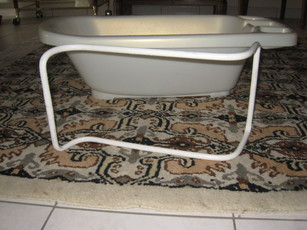
\includegraphics{baignoire.jpg}
  \end{tabular}
}




\end{document}

%%% Local Variables: 
%%% mode: latex
%%% TeX-master: t
%%% TeX-PDF-mode: t
%%% End: 
